\chapter{Resultados}\label{cap:resultados}

Os resultados decorrentes do desenvolvimento deste projeto foram:

\begin{itemize}
  \item Dados resultantes da comparação entre cinco diferentes inteligências e seu desepenho na extração de contextos relevantes presentes em dados de laboratórios e demandas coletados pelo \gls{direc} ao longo dos anos.
  \item A criação de uma aplicação capaz de integrar diferentes modelos de inteligência artificial para a análise linguistica de textos e extração de palavras-chave, bem como a análise de similiaridade entre contextos.
  \item A criação de uma aplicação capaz de mediar a utilização de uma aplicativo mobile com uma aplicação de análise de dados.
  \item Um \gls{mvp} mobile como prova de conceito na utilização das tecnologias empregadas, aceitando a entrada de dados de usuários e oferencendo resultados compreensíveis.
\end{itemize}

% ------------------------------------ Escopo do Sistema ------------------------------------ %
\section{Escopo do sistema}\label{sec:escopo}

O projeto Contrate um Cientista possui dois objetivos principais, sendo eles, a realização de uma análise comparativa entre diferentes modelos de linguagem na terefa de associação de demandas com laboratórios, e a facilitação da formação de parcerias entre o setor produtivo e a expertise científica presente nas universidades através de uma aplicação que, de forma inteligente e automatizada, norteie a tomada de decisões na formação de parcerias. Com estes objetvios postos, é necessaário realizar algumas considerações sobre o escopo do projeto.

O sistema desenvolvido não visa eliminar a necessidade de avaliação das sugestões realizadas pelos profissíonais responsáveis, mas sim fornecer uma ferramenta que auxilie na tomada de decisão, pois nenhum sistema é a prova de falhas. O aplicativo desensolvido é uma prova de conceito e não deve ser visto como uma solução pronta para ambiente de produção, pois mesmo que implemente um mecânismo básico de segurança, não foi desenvolvido com foco na segurança dos dados. Para um cenário de utilização real, a base de dados deve estar presente é um ambiente seguro com acesso controlado, e o armazenamento de dados de usuários deve seguir as regras impostas pela \gls{lgpd}.

As inteligências \gls{bert}, \gls{gpt}, Azure AI Language e Amazon Comprehend foram escolhidas por se tratar de modelos de linguagem desensolvidos pelas quatro gigantes na área de tecnologia e \gls{ia}, Google, OpenAI, Microsoft e Amazon, respectivamente. A inteligência \gls{yake}, mesmo sendo um modelo análitico, foi escolhido para efeitos de comparação entre \gls{llm} e modelos de análise de texto mais tradicionais. Outro fator que contribuiu para a escolha destas tecnologias foi a disponibilidade de uma \gls{api} de integração e facilidade de implementação.

O sistema abrange dois tipos de usuários, organizações e laboratórios. Ambos os tipos de usuário utilizaram a mesma tela de login para acesso à aplicação, sendo que o conteúdo apresentado após autenticação no sistema difere a depender do tipo de usuário. Organizações são responsáveis pela criação das demandas, cujo conteúdo é analisado contra as informações de todos os laboratórios cadastrados, gerando uma pontuação indicativa de similaridade para cada um. Organizações tambem seram capazes de favoritar os laboratórios de sua preferência por demanda. Laboratórios são responsáveis pelo cadastro de seus recursos relavantes, como descrição do trabalho que efetuam, equipamentos, softwares e certificados, que serão utilizados para a análise e podem ser visualizados pelas organizações.

Para realizar a comparação entre as inteligências integradas foi construído um projeto a parte de teste e benchmarking. Este projeto simula o consumo dos pontos de extremidade expostos pela \gls{api} de aplicação da mesma forma que o aplicativo mobile, porém obtendo informações relevantes para à análise de desempenho, como por exemplo, o tempo de análise de cada inteligência, armazenando as informações obtidas em um banco de dados. Estas informações são utilizadas na conclusão e ajudam a enteder os pontos positivos e possíveis melhorias que podem basear trabalhos futuros.

% ----------------------------------- Modelagem do Sistema ---------------------------------- %

\section{Modelagem do sistema}\label{sec:modelagem}

O processo de modelagem do sistema foi divido de modo a habilitar a compartimentalização através da separação de conceitos e tarefas que cada módulo deve atender, permitindo uma maior escalibidade e facilitando o processo de manutenção. Nesta seção estão identificados os requisitidos de cada aplicação e o projeto arquitetural de cada uma.

\subsection{Modelagem da Aplicação Mobile}\label{subsec:modelagem_app}

As tabelas \autoref{tab:requisitos_funcionais_app} e \autoref{tab:requisitos_nao_funcionais_app} apresentam os requisitos funcionais e não funcionais identificados para a aplicação mobile. No seu levantamento foram consideradas as necessidades dos usuários, sendo eles laboratórios e organizações, e os objetivos pretendidos pelo \gls{direc}.

\begin{table}[htb]
  \caption{Requisitos funcionais da aplicação mobile.}
  \label{tab:requisitos_funcionais_app}
  \begin{tabularx}{\textwidth}{l|l}
    \hline
    \textbf{Requisito} & \textbf{Descrição}                                                                    \\ \hline
    RF1                & O aplicativo deve permitir o cadastro de laboratórios                                 \\
    RF2                & O aplicativo deve permitir o cadastro de organizações                                 \\
    RF3                & O aplicativo deve permitir que usuários se autentiquem no sistema                     \\
    RF4                & O aplicativo deve permitir que o usuário visualize e edite o seu perfil               \\
    RF5                & O aplicativo deve permitir que uma organização crie uma demanda                       \\
    RF6                & O aplicativo deve permitir que uma organização atualize uma demanda                   \\
    RF7                & O aplicativo deve permitir que uma organização finalzie uma demanda                   \\
    RF8                & O aplicativo deve permitir que uma organização favorite laboratórios por demanda      \\
    RF9                & O aplicativo deve permitir a visualização das demandas de uma organização             \\
    RF10               & O aplicativo deve permitir a visualização das pontuações dos laboratórios por demanda \\
    RF11               & O aplicativo deve permitir a visualização das demandas de uma organização             \\ \hline
  \end{tabularx}
  \fonte{}
\end{table}

\begin{table}[htb]
  \caption{Requisitos não funcionais da aplicação mobile.}
  \label{tab:requisitos_nao_funcionais_app}
  \begin{tabularx}{\textwidth}{l|l}
    \hline
    \textbf{Requisito} & \textbf{Descrição}                                                          \\ \hline
    RNF1               & O aplicativo deve permitir ser instalado em sistema operacional Android     \\
    RNF2               & O aplicativo deve permitir ser instalado em sistema operacional iOs         \\
    RNF3               & O aplicativo deve ser implementado com o framework Flutter e linguagme Dart \\
    RNF4               & O aplicativo deve mascarar a senha do usuário na autenticação               \\
    RNF5               & O aplicativo deve ser capaz de se comunicar com \gls{api}'s externas        \\
    RNF6               & O aplicativo deve ter baixo impacto no armazenamento do dispositivo         \\
    RNF7               & O aplicativo deve ter uma interface intuitiva e de facil navegação          \\ \hline
  \end{tabularx}
  \fonte{}
\end{table}

Para representar os tipos de usuários e suas possíveis funções, temos os diagramas de casos de uso das \autoref{fig:caso-uso-org} e \autoref{fig:caso-uso-lab}.

\begin{figure}[htb]
  \captionsetup{width=0.43\textwidth}
  \caption{Diagrama de caso de uso da organização.}
  \label{fig:caso-uso-org}
  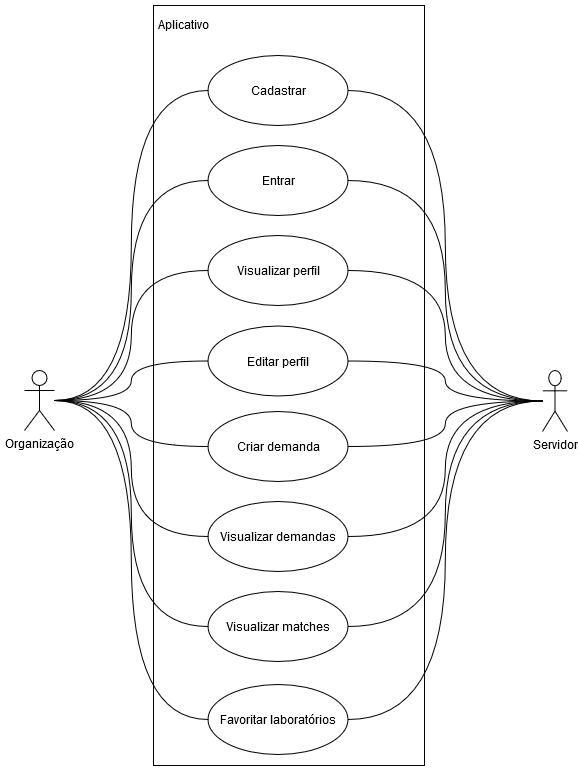
\includegraphics[scale=0.8]{caso-uso-org}
  \fonte{}
\end{figure}

\begin{figure}[htb]
  \captionsetup{width=0.43\textwidth}
  \caption{Diagrama de caso de uso da organização.}
  \label{fig:caso-uso-lab}
  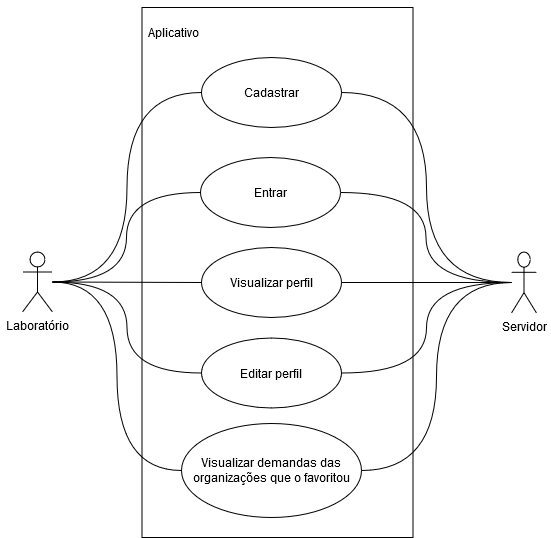
\includegraphics[scale=0.8]{caso-uso-lab}
  \fonte{}
\end{figure}

\subsection{Modelagem da API de Aplicação}\label{subsec:modelagem_api}

A \gls{api} de aplicação foi projetada para que possa ser integrada a qualquer sistema que seja capaz de realizar requisições \gls{http} através de uma arquitetura \gls{rest}. Também foi configurada para ser o agente responsável pela manipulação e persistência dos dados. As tabelas \autoref{tab:requisitos_funcionais_api} e \autoref{tab:requisitos_nao_funcionais_api} aprensentam os requisitos indentificados para esta aplicação.

\begin{table}[htb]
  \caption{Requisitos funcionais da Api de aplicação.}
  \label{tab:requisitos_funcionais_api}
  \begin{tabularx}{\textwidth}{l|l}
    \hline
    \textbf{Requisito} & \textbf{Descrição}                                                                        \\ \hline
    RF1                & A aplicação deve ser capaz de receber e responder requisições \gls{http}                  \\
    RF2                & A aplicação deve seguir a arquitetura \gls{rest}                                          \\
    RF3                & A aplicação deve ser capaz de se conectar a um banco de dados                             \\
    RF4                & A aplicação deve responder à requisições no formato \gls{json}                            \\
    RF5                & A aplicação deve ser capaz de receber requisições no formato \gls{json}                   \\
    RF6                & A aplicação deve ser capaz de autenticar um usuário utilizando Json Web Tokens            \\
    RF7                & Exceto pela autenticação e registro, endpoints só podem ser consumidos após autenticação  \\
    RF8                & A aplicação deve ser capaz de distinguir entre usuários do tipo laboratório e organização \\
    RF9                & Um usuário só poderá requisitar dados vinculados à seu tipo de usuário e conta            \\
    RF10               & A aplicação deve ser capaz de realizar requisições \gls{http} à \gls{api} de linguagem    \\ \hline
  \end{tabularx}
  \fonte{}
\end{table}

\begin{table}[htb]
  \caption{Requisitos não funcionais da Api de aplicação.}
  \label{tab:requisitos_nao_funcionais_api}
  \begin{tabularx}{\textwidth}{l|l}
    \hline
    \textbf{Requisito} & \textbf{Descrição}                                                                        \\ \hline
    RNF1               & A aplicação deve criptografar a senha de usuários antes de persistência no banco de dados \\
    RNF2               & A aplicação deve ser compatível com containeres do Docker                                 \\
    RNF3               & A aplicação deve ser implementada com o framework .NET e linguagem C{\#}                  \\
    RNF4               & A aplicação deve ser capaz de realizar escritas e leituras na base de dados               \\
    RNF5               & Todos os métodos implementados devem ser assincronos                                      \\ \hline
  \end{tabularx}
  \fonte{}
\end{table}

Para atender a todos os possíveis casos de uso, a \gls{api} de aplicação foi subdividida em cinco subdomínios sendo eles:

\begin{itemize}
  \item \textbf{auth}: Responsável pela autenticação de usuários;
  \item \textbf{match}: Responsável pela consulta e marcação de favoritos entre demandas e laboratórios.
  \item \textbf{demand}: Responsável pela criação, atualização, finalização e consulta de demandas.
  \item \textbf{company}: Responsável pela criação e obtenção de dados de usuários do tipo organização.
  \item \textbf{laboratory}: Responsável pela criação e obtenção de dados de usuários do tipo laboratório.
\end{itemize}

Como fora descrito nos requisitos funcionais, a aplicação é também responsável pelas transações com o banco de dados. O diagrama da figura \ref{fig:ERD} apresenta as entidades que foram criadas e a forma como se relacionam para atender as necessidades do sistema.

\begin{figure}[htb]
  \captionsetup{width=0.43\textwidth}
  \caption{Diagrama de Relação de Entidades do Bando de Dados.}
  \label{fig:ERD}
  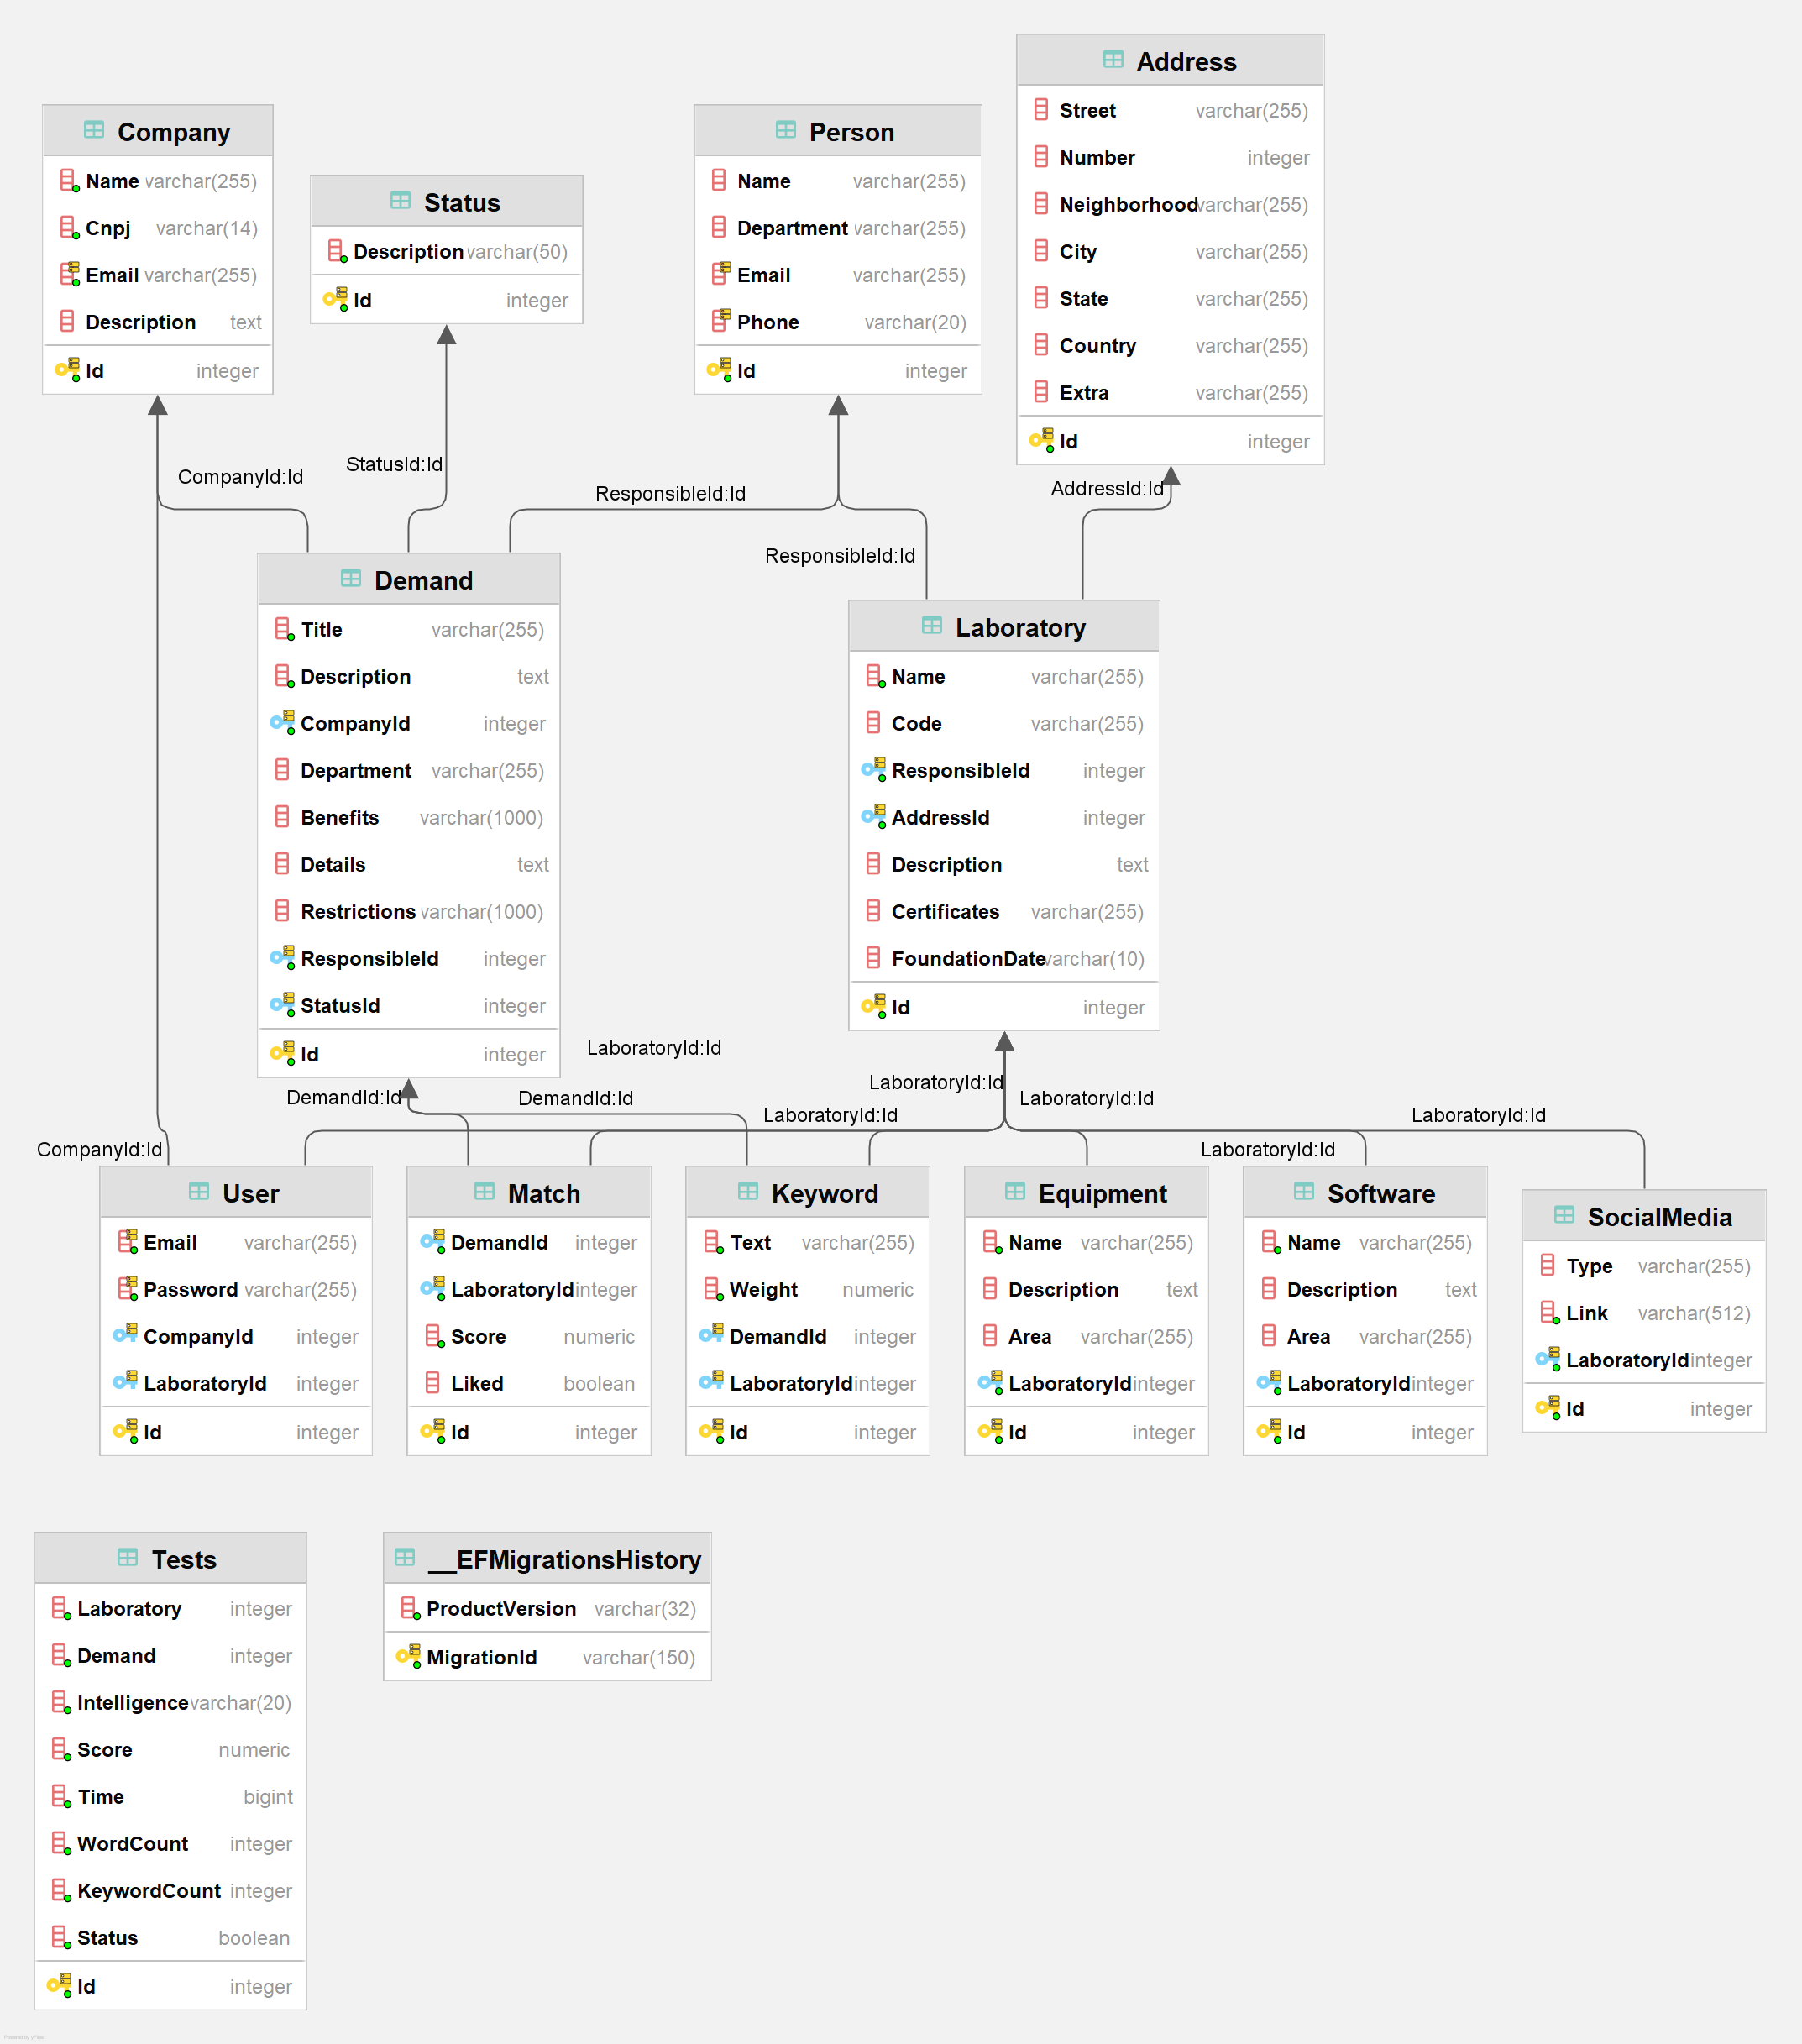
\includegraphics[scale=0.5]{ERD}
  \fonte{}
\end{figure}

\subsection{Modelagem da API de Linguagem}\label{subsec:modelagem_linguagem}

De forma similar à \gls{api} de aplicação, a \gls{api} de linguagem também foi projetada com o intuito de poder ser integrada a qualquer sistema que seja capaz de realizar requisições \gls{http} através de uma arquitetura \gls{rest}. Foi modelada para análisar as informções somente no momento de sua requisição, portanto é independente do contexto do agente que a consome e não realiza nenhum tipo de persistência de dados por si só. As tabelas \autoref{tab:requisitos_funcionais_linguagem} e \autoref{tab:requisitos_nao_funcionais_linguagem} apresentam os requisitos indentificados para esta aplicação.

\begin{table}[htb]
  \caption{Requisitos funcionais da pi de linguagem.}
  \label{tab:requisitos_funcionais_linguagem}
  \begin{tabularx}{\textwidth}{l|l}
    \hline
    \textbf{Requisito} & \textbf{Descrição}                                                             \\ \hline
    RF1                & A aplicação deve ser capaz de receber e responder requisições \gls{http}       \\
    RF2                & A aplicação deve seguir a arquitetura \gls{rest}                               \\
    RF4                & A aplicação deve responder à requisições no formato \gls{json}                 \\
    RF5                & A aplicação deve ser capaz de receber requisições no formato \gls{json}        \\
    RF6                & A aplicação deve ser capaz de autenticar um usuário utilizando Json Web Tokens \\
    RF7                & Exceto pela autenticação, endpoints só podem ser consumidos após autenticação  \\
    RF8                & A aplicação não deve persistir nenhum dado após execução                       \\
    RF9                & As chaves de autentição com as inteligenências devem ser informadas
    somente na criação da aplicação                                                                     \\
    RF9                & As lógicas de extração e análise devem ser segregadas                          \\ \hline
  \end{tabularx}
  \fonte{}
\end{table}

\begin{table}[htb]
  \caption{Requisitos não funcionais da api de linguagem.}
  \label{tab:requisitos_nao_funcionais_linguagem}
  \begin{tabularx}{\textwidth}{l|l}
    \hline
    \textbf{Requisito} & \textbf{Descrição}                                                           \\ \hline
    RNF2               & A aplicação deve ser compatível com containeres do Docker                    \\
    RNF3               & A aplicação deve ser implementada com o framework FastAPI e linguagem Python \\
    RNF5               & Todos os métodos implementados devem ser assincronos                         \\ \hline
  \end{tabularx}
  \fonte{}
\end{table}

Sendo as funções da aplicação de análise de similaridade e extração de palavras-chave, a \gls{api} foi dividida em três subdomínios:

\begin{itemize}
  \item \textbf{auth}: Responsável pela autenticação de usuários.
  \item \textbf{analyze}: Responsável pela análise de similaridade entre textos.
  \item \textbf{extract}: Responsável pela extração de palavras-chave de um texto utilizando uma inteligência específica.
\end{itemize}

% --------------------------------- Apresentação do Sistema --------------------------------- %

\section{Apresentação do sistema}\label{sec:apresentacao}

Para uma representação visual do fluxo e da estrutura de interação entre todas as páginas do sistema, é utilizado o diagrama de navegação na \autoref{fig:diagrama-navegacao}, onde mostra como os usuários navegarão de uma tela para outra.

\begin{figure}[htb]
  \captionsetup{width=0.43\textwidth}
  \caption{Diagrama de navegação de telas do aplicativo.}
  \label{fig:diagrama-navegacao}
  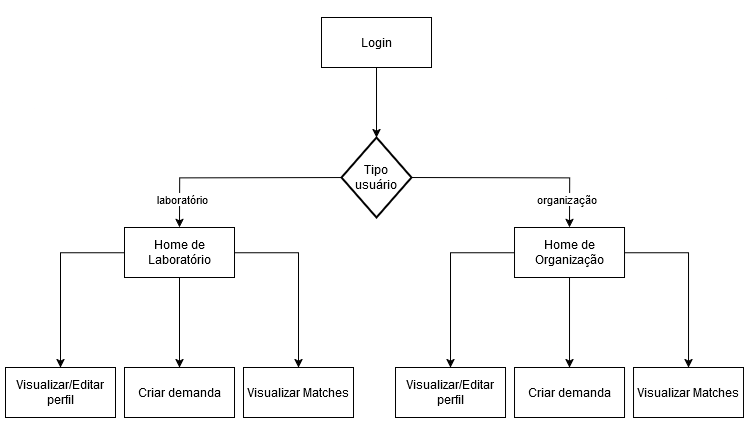
\includegraphics[scale=0.8]{diagrama-navegacao}
  \fonte{}
\end{figure}

O sistema possui uma tela para entrar inicialmente, onde o usuário pode preencher seu email e senha, ou fazer seu registro. Antes de realizar o signin, o usuário precisa escolher se ele é um laboratório ou organização a se registrar, e então ele é direcionado para seu respectivo formulário para preencher com suas informações. As telas para entrar e se cadastrar nos sistemas estão representadas na \autoref{fig:pagina-login-signin}.

\begin{figure}[htb]
  \captionsetup{width=0.43\textwidth}
  \caption{Tela para entrar e se registrar do aplicativo.}
  \label{fig:pagina-login-signin}
  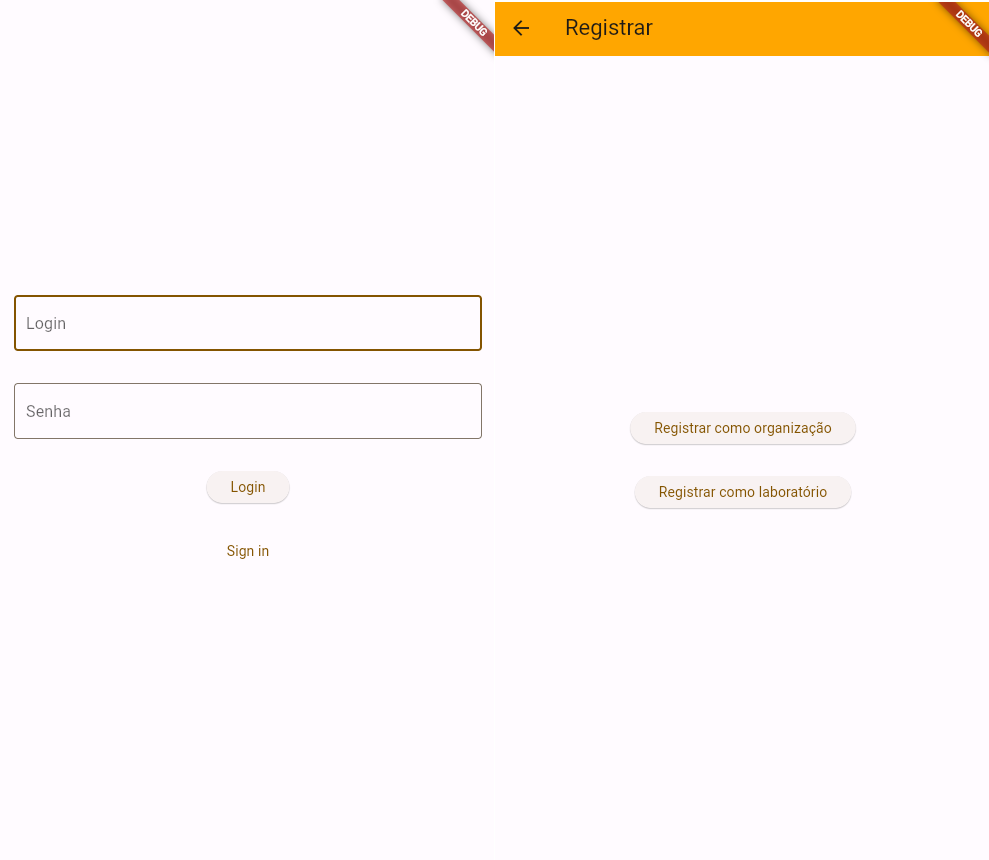
\includegraphics[scale=0.6]{pagina-login-signin}
  \fonte{}
\end{figure}

Após realizar o login e senha, o usuário será redirecionado para sua tela principal, á esquerda da \autoref{fig:pagina-home} está a tela para um usuário do tipo organização, e á direita, para um usuário do tipo laboratório.

\begin{figure}[htb]
  \captionsetup{width=0.43\textwidth}
  \caption{Telas iniciais de um usuário do tipo organização e laboratório, respectivamente, do aplicativo.}
  \label{fig:pagina-home}
  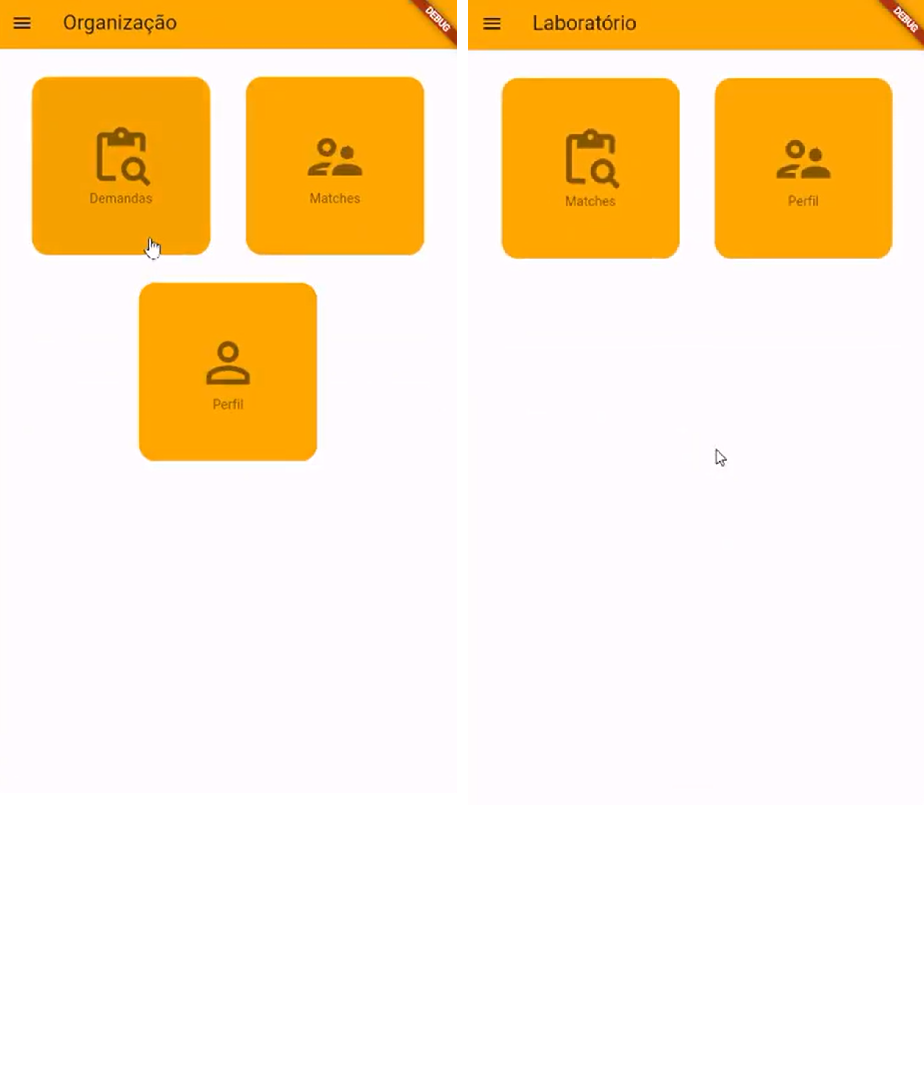
\includegraphics[scale=0.6]{pagina-home}
  \fonte{}
\end{figure}

Ou seja, uma organização poderá ver seu perfil, as demandas e os ranqueamentos de todos os laborátorios para cada demanda, além dos seus detalhes, demonstrado pela, enquanto o laboratório poderá ver seu perfil e os matches com os detalhes da demanda do organizador que o marcou como favorito.

A tela de perfil, é onde o usuário poderá visualizar e editar todas as suas informações de perfil, na \autoref{fig:pagina-form-perfil} temos essas telas de organização e laboratório, respectivamente. Esse mesmo formulário, é visível ao se registrar no aplicativo.

\begin{figure}[htb]
  \captionsetup{width=0.43\textwidth}
  \caption{Tela de detalhes de perfil da organização e laboratório, respectivamente, do aplicativo.}
  \label{fig:pagina-form-perfil}
  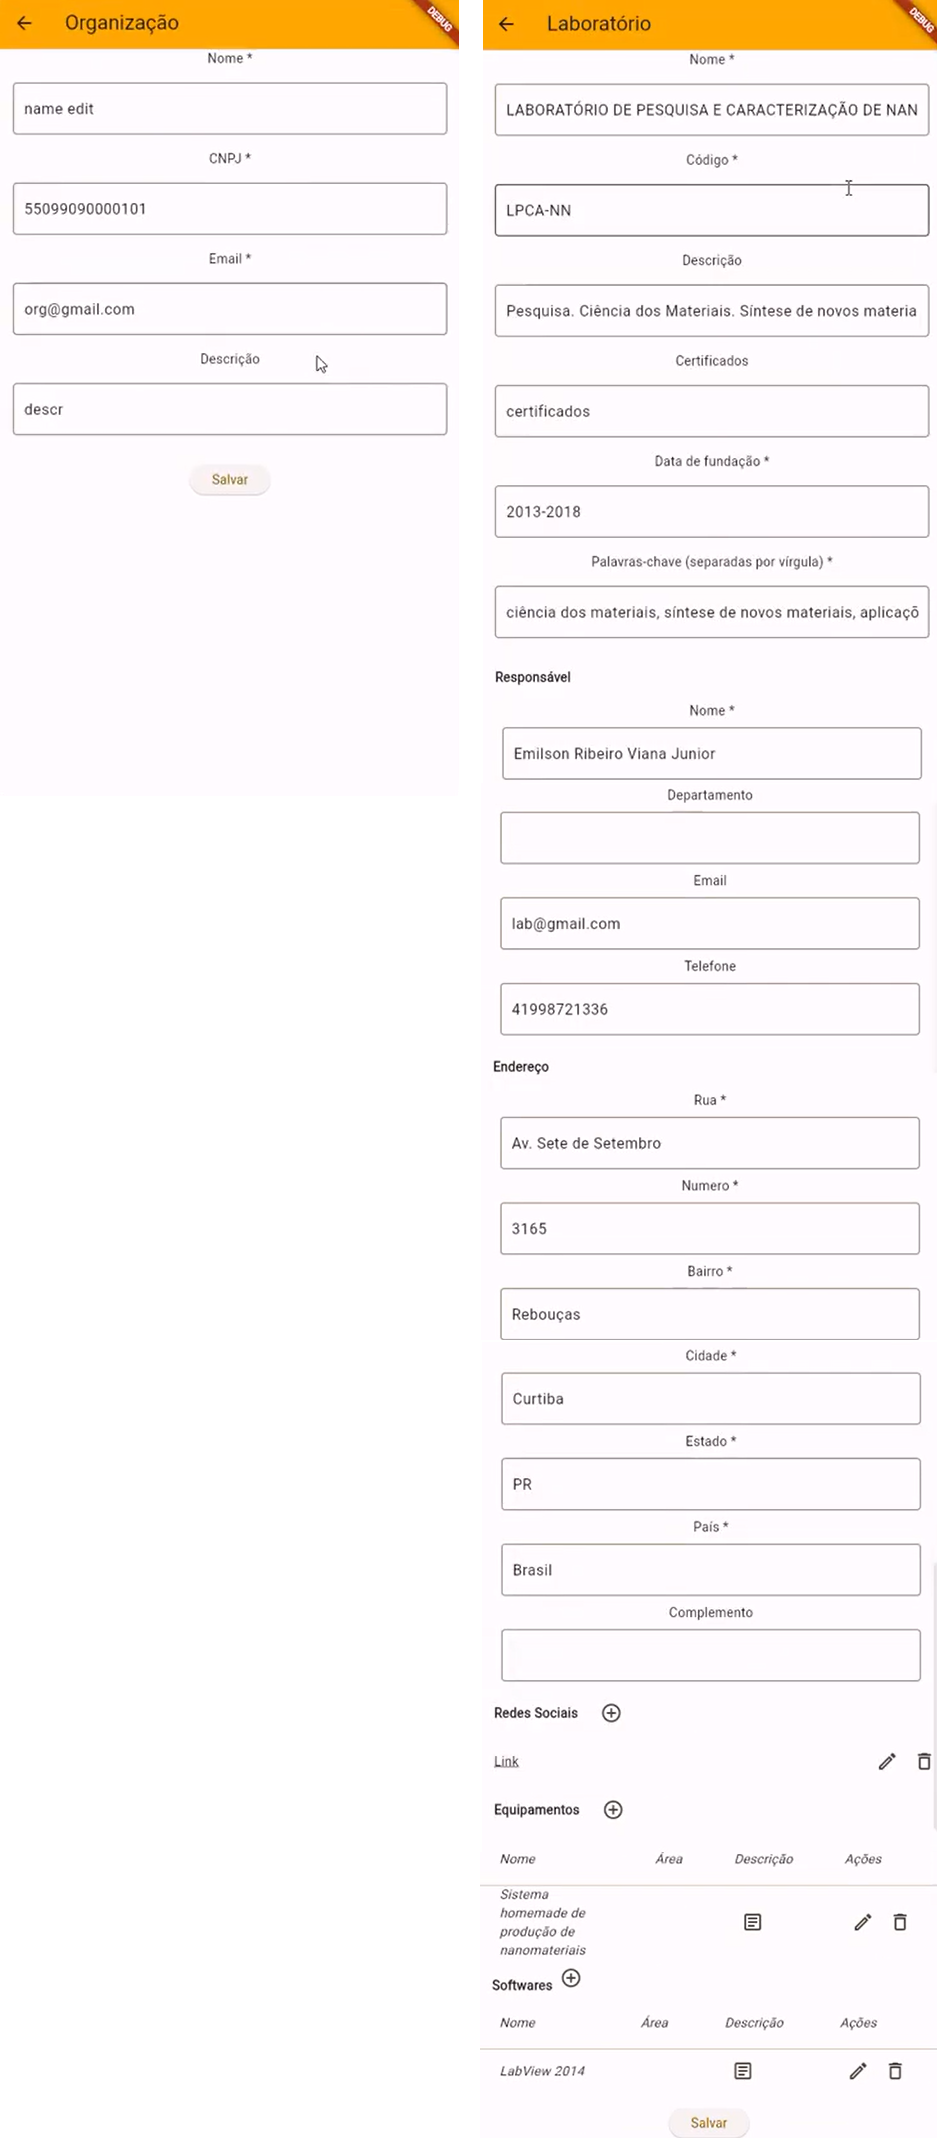
\includegraphics[scale=0.4]{pagina-form-perfil}
  \fonte{}
\end{figure}

As páginas das demandas na \autoref{fig:paginas-demanda}, podem ser gerenciadas apenas para usuários do tipo organização. E é possível visualizar uma lista com todas as demandas já cadastradas, editar a demanda apenas se nenhum laboratório estiver associada a ela, visualizar os detalhes da demanda, e criar uma demanda nova.

\begin{figure}[htb]
  \captionsetup{width=0.43\textwidth}
  \caption{Telas de lista de demandas, detalhe de demanda e criação de demanda, respectivamente, do aplicativo.}
  \label{fig:paginas-demanda}
  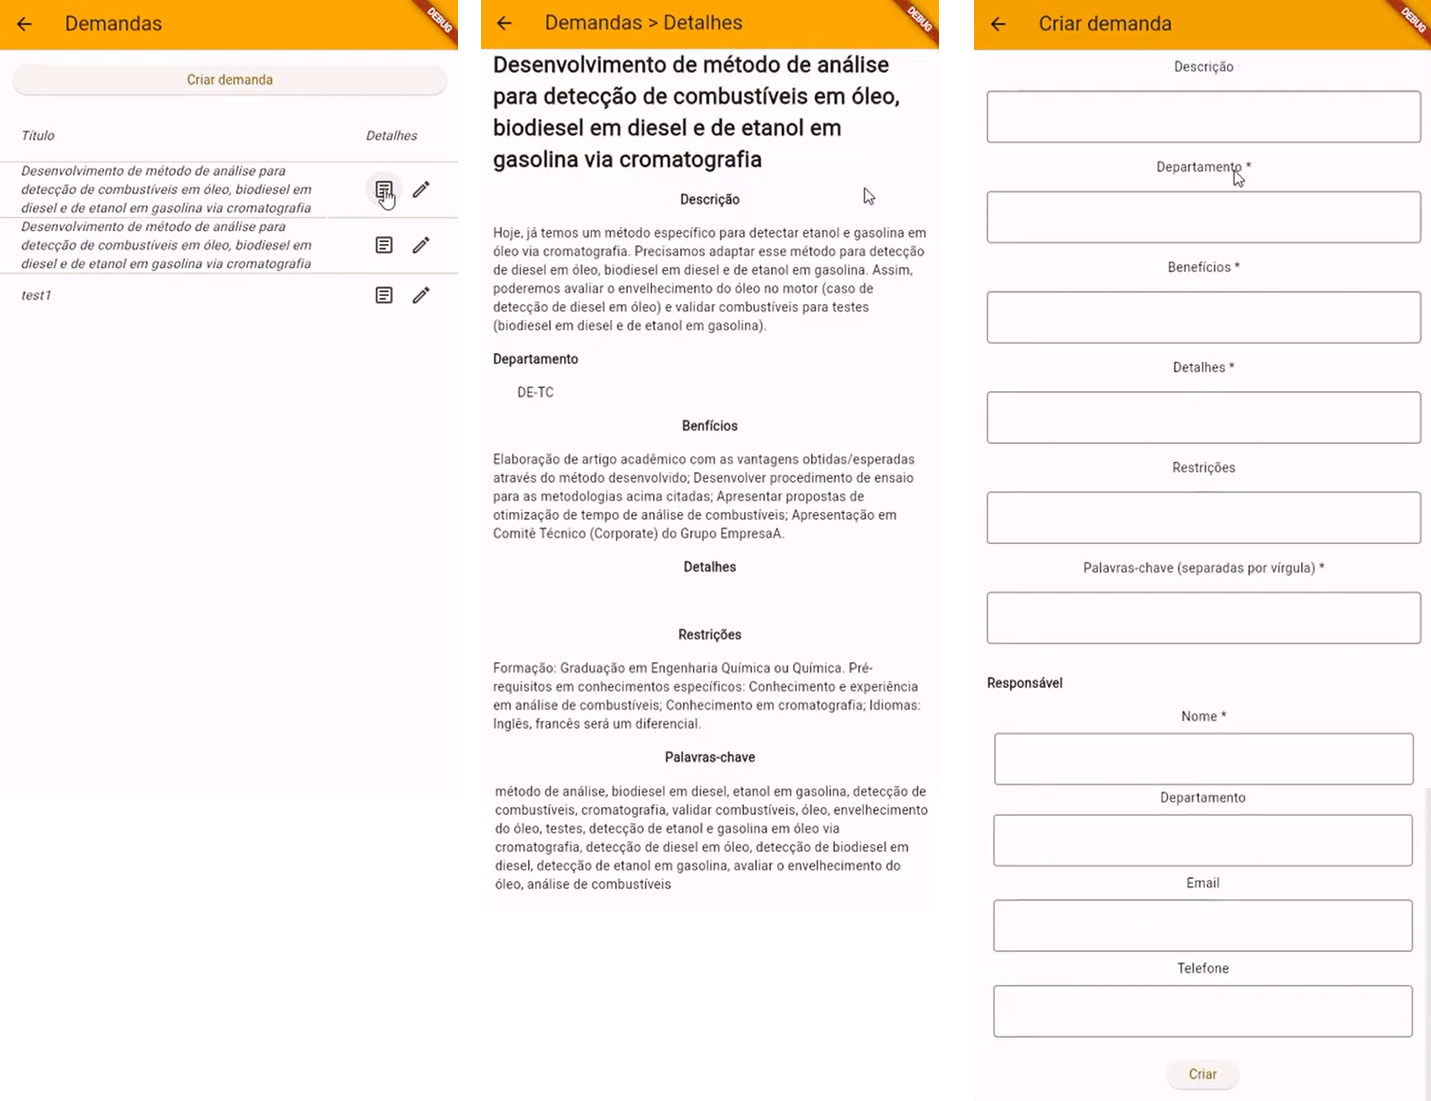
\includegraphics[scale=0.4]{paginas-demanda}
  \fonte{}
\end{figure}

Uma lista comum para ambos os usuários, é a tela de lista dos matches na \autoref{fig:pagina-matches}, onde é pode-se ver os detalhes daquela match.

\begin{figure}[htb]
  \captionsetup{width=0.43\textwidth}
  \caption{Tela da lista de matches do aplicativo.}
  \label{fig:pagina-matches}
  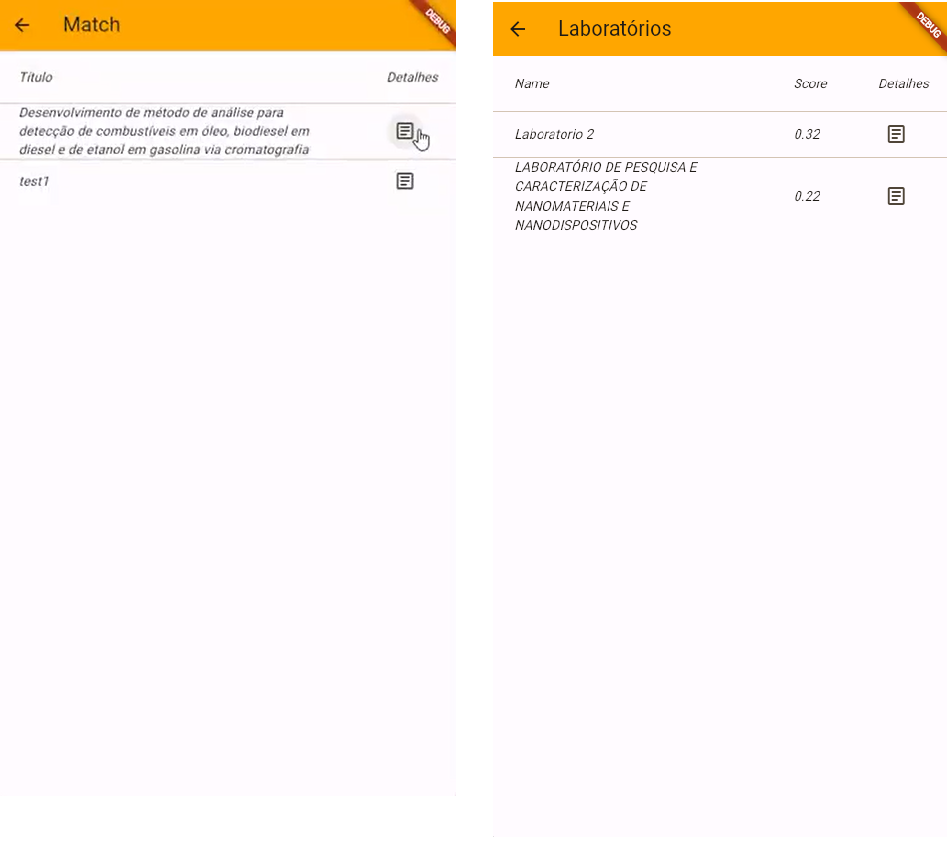
\includegraphics[scale=0.6]{pagina-matches}
  \fonte{}
\end{figure}

Para o usuário organização, ao clicar para visualizar os detalhes do match, ele tem acesso a todas as informações do laboratório que deu match com aquela demanda, e as descrições de equipamentos e softwares são visiveis através de um modal. Além dos detalhes, a organização pode marcar aquele laboratório como apto para aquela demanda, o que faz com que no aplicativo do laboratóio, ele possa ver os detalhes dessa demanda na respectiva tela. Já para o usuário laboratório, o botão de detalhes o leva para visualizar as informações completas da demanda. Ambas as página são mostradas na \autoref{fig:pagina-match}, e o título das duas páginas de detalhes, é o título da demanda em questão.

\begin{figure}[htb]
  \captionsetup{width=0.43\textwidth}
  \caption{Telas de detalhes de um match, com os detalhes do laboratório, assim como a descrição do equipmanto, de um usuário do tipo organização do aplicativo. E a tela de detalhe da demanda visualizado no aplicativo de laboratórios, com detalhes da demanda.}
  \label{fig:pagina-match}
  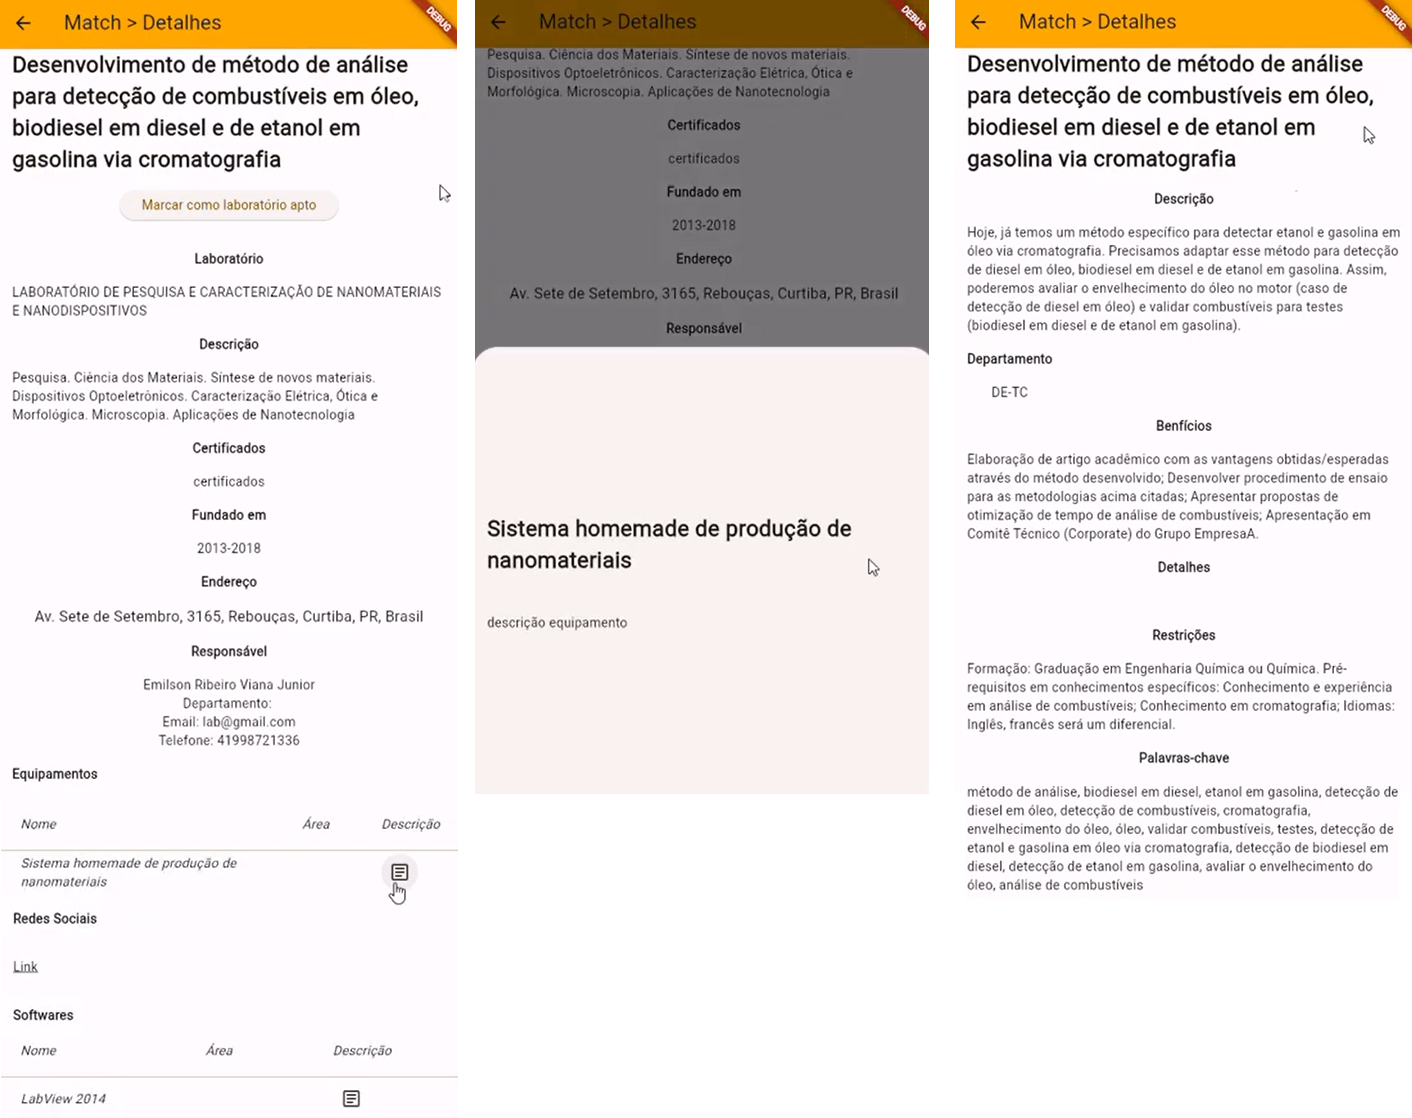
\includegraphics[scale=0.4]{pagina-match}
  \fonte{}
\end{figure}

% --------------------------------- Implementação do Sistema -------------------------------- %

\section{Implementação do sistema}\label{sec:implementacao}

\subsection{Implementação da Aplicação Mobile}\label{subsec:aplicacao}

A aplicação foi desenvolvida em Flutter, um framework, que utiliza o Dart como linguagem de programação. A interface é construída com componentes de interface para compor as páginas. Os componentes foram criados e organizados de forma independente, visando facilitar futuras implementações e alterações. Como por exemplo na \autoref{codigo:equip-form}, o componente de formulário do equipamento, que pode ser utilizado em diferentes páginas. O formulário é utilizado tanto para edição, quando para criação de equipamentos, e possui o campo "Nome" obrigatório, enquanto os campos "Descrição" e "Área" são opcionais. Quando pressionado o botão para salvar, o modal é fechado e os controllers são retornados populados para a página de lista de equipamentos, que salva os dados no banco de dados.

\begin{sourcecode}[htb]
  \caption{\label{codigo:equip-form}Componente do formulário de equipamentos}
  \begin{lstlisting}[frame=single, language=Java]
class EquipmentFormPage extends StatelessWidget {
  EquipmentFormPage(
      {Key? key,
      required this.nameController,
      required this.descriptionController,
      required this.areaController})
      : super(key: key);

  ...

  @override
  Widget build(BuildContext context) {
    return Scaffold(
      body: Form(
        key: _formKey,
        child: Column(mainAxisAlignment: MainAxisAlignment.center, children: [
          const Text('Nome *'),
          Padding(
            padding: const EdgeInsets.symmetric(horizontal: 16, vertical: 16),
            child: TextFormField(
              decoration: const InputDecoration(border: OutlineInputBorder()),
              controller: nameController,
              validator: (value) {
                if (value == null || value.isEmpty) {
                  return 'Por favor, insira um nome';
                }
                return null;
              },
            ),
          ),
		  
          ...
		  
          Padding(
            padding: const EdgeInsets.symmetric(horizontal: 16, vertical: 16),
            child: ElevatedButton(
              child: const Text('Salvar'),
              onPressed: () {
                Navigator.pop(context, true);
              },
            ),
          ),
\end{lstlisting}
  \fonte{}
\end{sourcecode}

Para a comunicação com a API de Aplicação, foi utilizada o pacote nativo http, onde é possível fazer todas as requições, com todos os parâmetros necessários. Entre esses parâmetros, está o token utilizado para a autenticação da rota. O token é registrado ao realizar o login no armazenamento interno, utilizando o pacote Shared Preferences, e sendo possível buscá-lo em todas as requisições. Abaixo na \autoref{codigo:list-demands}, é possível visualizar um trecho do código utilizada para buscar as desmandas da organização logada.

\begin{sourcecode}[htb]
  \caption{\label{codigo:list-demands}Buscar lista de demandas}
  \begin{lstlisting}[frame=single, language=Java]
static Future<List<Demand>?> getDemand() async {
    try {
      var url = Uri.parse(
          '${ApiConstants.baseUrl}${ApiConstants.demandEndpoint}/list');
		  
	  // buscar token
      final SharedPreferences prefs = await SharedPreferences.getInstance();
      final String? token = prefs.getString('token');
	  
	  // faz requisição das demandas daquela organização
      var response =
          await http.get(url, headers: {'Authorization': 'Bearer $token'});
      if (response.statusCode == 200) {
        var body = json.decode(response.body);

		// retorna a lista de demandas
        return List<Demand>.from(body.map((item) => Demand.fromMap(item)));
      }
    } catch (e) {
	  throw Exception(e.toString());
    }
}
\end{lstlisting}
  \fonte{}
\end{sourcecode}

Por falta de disponibilidade de um equipamento com sistema operacional macOS, o aplicativo foi desenvolvido apenas para a plataforma Android. Atualmente, ele conta com um arquivo instalador que precisa ser transferido para o celular para permitir a instalação direta no dispositivo. No futuro, se faz necessário disponibilizá-lo na Google Play Store, a fim de simplificar o processo de instalação e oferecer maior praticidade aos usuários.

\subsection{Implementação da API de Aplicação}\label{subsec:api-aplicacao}

Como descrito nas seções \ref{subsec:app_api} e \ref{subsec:modelagem_api} a \gls{api} de aplicação possui quinze rotas organizadas em cinco subdomínios. O ponto inicial de interação de um usuário com a aplicação são as rotas de registro, tanto para laboratórios quanto para organizações.

O subdomínio de laboratórios possui três rotas:

\begin{itemize}
  \item \texttt{GET /laboratory}
  \item \texttt{POST /laboratory/register}
  \item \texttt{PUT /laboratory/update}
\end{itemize}

A rota \texttt{/register} espera um corpo de requisição como descrito no códido \ref{codigo:register-lab}.

\begin{sourcecode}[htb]
  \caption{\label{codigo:register-lab}Corpo JSON de registro de laboratório}
  \begin{lstlisting}[frame=single, language=Java]
{
  "name": "string",
  "code": "string",
  "description": "string",
  "certificates": "string",
  "foundationDate": "DateTime",
  "responsible": {
    "name": "string",
    "email": "string",
    "password": "string",
    "departament": "string",
    "phone": "string"
  },
  "address": {
    "street": "string",
    "number": int,
    "neighborhood": "string",
    "city": "string",
    "state": "string",
    "country": "string",
    "extra": "string"
  },
  "softwares": [
    {
      "name": "string",
      "description": "string",
      "area": "string"
    }
  ],
  "equipments": [
    {
      "name": "string",
      "description": "string",
      "area": "string"
    }
  ],
  "socialMedias": [
    {
      "type": "string",
      "link": "string"
    }
  ],
  "keywords": [
    "keyword 1",
    "keyword 2"
  ]
}
\end{lstlisting}
  \fonte{}
\end{sourcecode}

O consumo deste endpoint engatilha a chamada de extração de palavras-chave utilizando a inteligência configurada no início da aplicação. O código \ref{codigo:analyze-lab} representa o método que recebe a requisição, a deserializa e chama o endpoint da \gls{api} de linguagem para realizar a extração. Este método também realiza algumas validações antes de prosseguir com o processamento, como a garantia de que o laboratório com o email informado já não esteja cadastrado, de que a senha informada possua pelo menos 8 caracteres com pelo menos um número e uma letra e que o campo descrição, utilizado na extração de contexto, esteja preenchido.

\begin{sourcecode}[htb]
  \caption{\label{codigo:analyze-lab}Método de registro e análise de laboratório}
  \begin{lstlisting}[frame=single, language=Java]
public async Task<LoginResponse> Register(Laboratory laboratory)
{
  // Verifica se o e-mail já está cadastrado
  BadRequestException.ThrowIf 
  (
      await userRepository.ExistsAsync(laboratory.Responsible.Email), 
      "E-mail já cadastrado."
  );

  // Verifica se a senha é válida
  BadRequestException.ThrowIf
  (
      !ValidationHelper.ValidatePassword(laboratory.Responsible.Password), 
      "Senha inválida. A senha deve conter pelo menos 8 caracteres, 
      uma letra e um número."
  );

  // Verifica se a descrição do laboratório foi informada
  BadRequestException.ThrowIf
  (
      string.IsNullOrEmpty(laboratory.Description), 
      "A descrição do laboratório é obrigatória."
  );

  // Extrai as palavras-chave da descrição do laboratório
  var keywords = await languageService.Extract
  (
      new Description { Text = laboratory.Description }
  );

  // Cria o usuário, concatena as palavras-chave extraídas 
  // com as informadas e insere no banco de dados
  var user = await userRepository.InsertAsync(
      (keywords, laboratory).Adapt<User>()
  );

  // Cria o token de autenticação
  var token = tokenService.Create(user);

  return (user, token).Adapt<LoginResponse>();
}
\end{lstlisting}
  \fonte{}
\end{sourcecode}

É importante notar que na chamada do método é permitido ao usuário informar uma lista de palavras-chave. Essas palavras-chave são agrupadas às extraídas pela inteligência e armazenadas no banco de dados, para que sempre que necessário possam ser utilizadas na análise de similaridade.

O subdomínio de empresas também possui três rotas:

\begin{itemize}
  \item \texttt{GET /company}
  \item \texttt{POST /company/register}
  \item \texttt{PUT /company/update}
\end{itemize}

A rota \texttt{/register} espera um corpo de requisição como descrito no códido \ref{codigo:register-company}.

\begin{sourcecode}[htb]
  \caption{\label{codigo:register-company}Corpo JSON de registro de empresas}
  \begin{lstlisting}[frame=single, language=Java]
{
  "name": "string",
  "cnpj": "string",
  "email": "string",
  "password": "string",
  "description": "string"
}
\end{lstlisting}
  \fonte{}
\end{sourcecode}

O registro de empresas não engatilha a extração de palavras-chave, pois para usuários do tipo empresa isso só ocorre na criação ou atualização de uma demanda.

Com um usuário já cadastrado, é possível se autenticar no sistema através da rota \texttt{/auth/login}, que espera um corpo de requisição como descrito no códido \ref{codigo:login}. O token gerado é utilizado para autenticar as requisições nas rotas protegidas.

\begin{sourcecode}[htb]
  \caption{\label{codigo:login}Corpo JSON da rota de login}
  \begin{lstlisting}[frame=single, language=Java]
Requisição
{
  "email": "string",
  "password": "string"
}

Resposta
{
	"userId": int,
	"userType": int,
	"type": "Bearer",
	"token": "string",
	"expires": 86400000
}
\end{lstlisting}
  \fonte{}
\end{sourcecode}

Outro subdomínio importante é o de demandas, composto por cinco rotas:

\begin{itemize}
  \item \texttt{POST /demand/create}
  \item \texttt{PUT /demand/update}
  \item \texttt{PUT /demand/finalize}
  \item \texttt{GET /demand/{id}}
  \item \texttt{GET /demand/list}
\end{itemize}

Os métodos \texttt{/create} e \texttt{/update} são especialmente relevantes pois engatilham a extração de palavras-chave. As rotas deste subdomínio só podem ser consumidos por usuários do tipo empresa. O códifo \ref{codigo:create-demand} apresenta o corpo de requisição esperado pela rota de criação e atualização de demandas.

\begin{sourcecode}[htb]
  \caption{\label{codigo:create-demand}Corpo JSON de registro de demandas}
  \begin{lstlisting}[frame=single, language=Java]
{
  "title": "string",
  "description": "string",
  "department": "string",
  "benefits": "string",
  "details": null,
  "restrictions": "string",
  "responsible": {
      "name": "string",
      "email": "string",
      "departament": "string",
      "phone": "string"
  },
  "keywords": [
      "Keyword 1",
      "Keyword 2"
  ]
}
\end{lstlisting}
  \fonte{}
\end{sourcecode}

Assim como no registro de laboratórios, a criação de demandas também engatilha a extração de palavras-chave das informações contidas na requisição, porém para demandas, a aplicação também realiza a chamada de análise de similaridade entre o texto da demanda e as palavras chaves de cada laboratório cadastrado. O código \ref{codigo:demand-analyze} apresenta o método que realiza a criação e a análise de demandas.

\begin{sourcecode}[htb]
  \caption{\label{codigo:demand-analyze}Método de cadastro e análise de demandas}
  \begin{lstlisting}[frame=single, language=Java]
public async Task<CreateDemandResponse> Create(CreateDemand createDemand)
{
    // Obtém o usuário realizando a requisição
    var user = await userService.GetUserAsync();

    // Verifica se o usuário é do tipo empresa
    ForbiddenException.ThrowIfNull
    (
        user.Company, 
        "Usuário não possui permissão para criar demandas"
    );

    // Carrega os dados necessários para a criação da demanda
    var status = await statusRepository.SelectAsync();
    var laboratories = await laboratoryRepository.SelectAsync();
    var person = await personRepository.GetAsync
    (
        createDemand.Responsible.Email, 
        createDemand.Responsible.Phone
    )

    // Extrai as palavras-chave das informações da demanda
    var keywords = await languageService.Extract
    (
        createDemand.Adapt<Description>()
    );

    // Realiza a análise de similaridade entre a demanda e os laboratórios
    var analysis = await languageService.Analyze
    (
        (createDemand, laboratories).Adapt<Analyze>()
    );

    // Persiste a demanda no banco de dados
    var demand = 
    (
        createDemand, 
        user, 
        person, 
        status, 
        keywords, 
        laboratories, 
        analysis
    ).Adapt<Demand>();

    await demandRepository.InsertAsync(demand);

    return (demand, laboratories, analysis).Adapt<CreateDemandResponse>();
}
\end{lstlisting}
  \fonte{}
\end{sourcecode}

Por fim, o útlimo subdomínio é o de matches, composto por três rotas:

\begin{itemize}
  \item \texttt{GET /match/{id}}
  \item \texttt{GET /match/list}
  \item \texttt{POST /match/like}
\end{itemize}

O método \texttt{/like} é utilizado por uma empresa para marcar um laboratório como possível candidato para uma demanda. O método \texttt{/list} pode ser utilizado por ambos os tipos de usuários e de algumas maneiras. Este método aceita algumas informações de filtro na query, sendo eles:

\begin{itemize}
  \item \texttt{/match/list}
        \begin{itemize}
          \item Quando chamado por um usuário do tipo laboratório, retorna todas as demandas que foram marcadas como favoritas para ele.
          \item Quando chamada por um usuário do tipo empresa, retorna todas as demandas da empresa, contendo todos os laborátorios e seus respectivos scores para cada demanda.
        \end{itemize}
  \item \texttt{/match/list?demand=id}: Onde id é uma demanda específica.
        \begin{itemize}
          \item Quando chamado por um usuário do tipo laboratório, retorna a demanda caso tenha sido favoritado.
          \item Quando chamada por um usuário do tipo empresa, retorna a demanda da empresa, contendo todos os laborátorios e seus respectivos scores.
        \end{itemize}
  \item \texttt{/match/list?laboratory=id}: Onde id é um laboratório específico.
        \begin{itemize}
          \item Quando chamado por um usuário do tipo laboratório, retorna todas as demandas que foram marcadas como favoritas para ele.
          \item Quando chamada por um usuário do tipo empresa, retorna as demandas da empresa, contendo o laborátorio e seus respectivos scores para cada demanda.
        \end{itemize}
  \item \texttt{/match/list?demand=id\_demand\&laboratory=id\_lab}: Onde \texttt{id\_demand} é uma demanda específica e \texttt{id\_lab} é um laboratório específico.
        \begin{itemize}
          \item Quando chamado por um usuário do tipo laboratório, retorna a demanda caso tenha sido favoritada.
          \item Quando chamada por um usuário do tipo empresa, retorna a demanda da empresa, contendo o laborátorio e seu respectivo score para a demanda.
        \end{itemize}
\end{itemize}

O diagrama da figura \ref{fig:api_aplicacao} apresenta os relacioanamentos básicos que a aplicação possui com o resto do sistema.

\begin{figure}[htb]
  \caption{Diagrama de bloccos da API de Aplicação}
  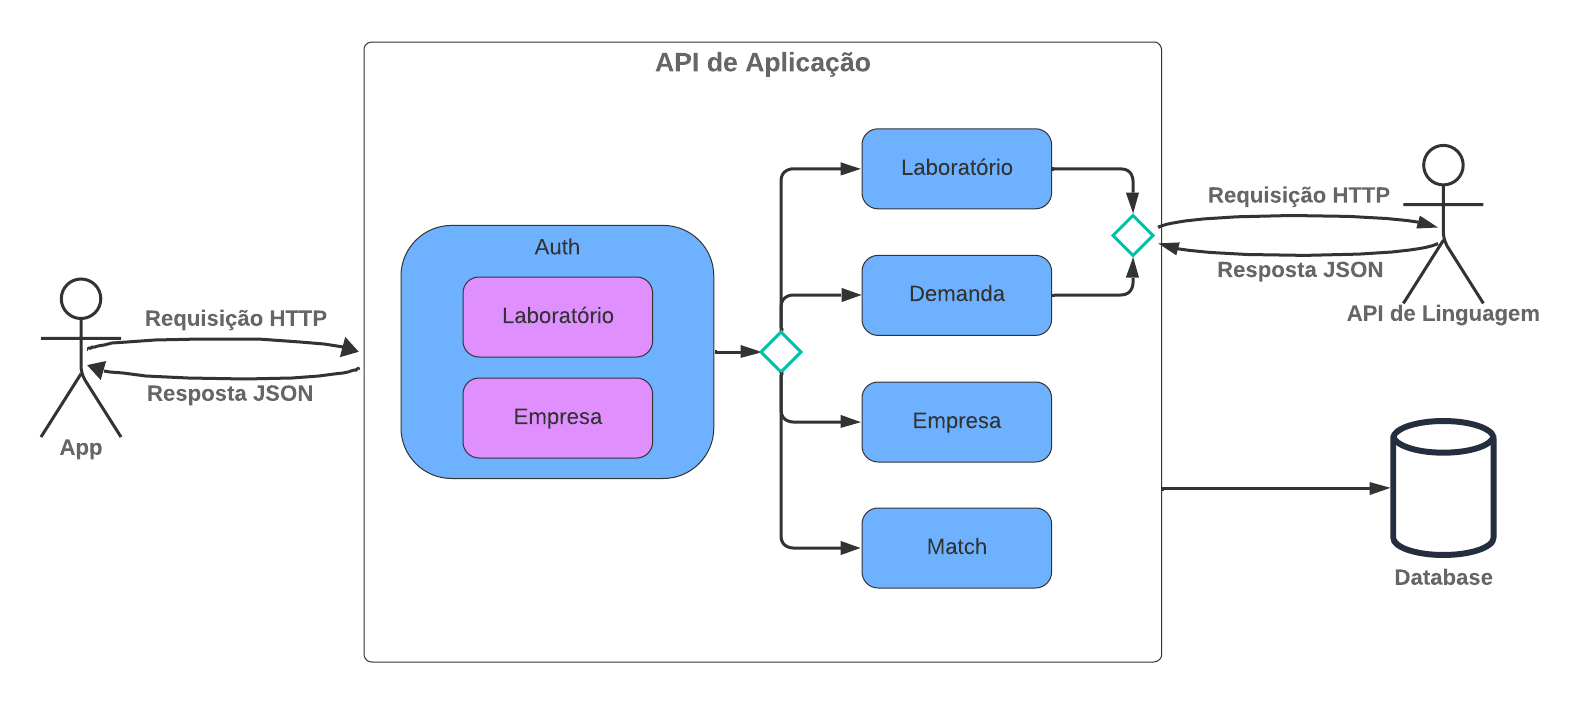
\includegraphics[scale=0.65]{api-aplicacao}
  \fonte{Autoria própria (2025)}
  \label{fig:api_aplicacao}
\end{figure}

\subsection{Implementação da API de linguagem}\label{subsec:api-linguagens}

Como descrito nas seções \ref{subsec:language_api} e \ref{subsec:modelagem_linguagem} a \gls{api} de linguagem possui sete rotas organizadas em três subdomínios. Antes que quaisquer requisições possam ser realizadas, é necessário a autenticação do sistema requisitor, através da rota \texttt{/auth/login}. Esta rota espera um email e senha pré configurados no inicio da aplicação, e retorna um token de autenticação que deve ser utilizado em todas as requisições.

O segundo subdomínio é o de extração de palavras-chave, \texttt{/extract}, composto por cinco rotas, uma para cada inteligência integrada:

\begin{itemize}
  \item \texttt{POST /extract/aws}
  \item \texttt{POST /extract/gpt}
  \item \texttt{POST /extract/bert}
  \item \texttt{POST /extract/yake}
  \item \texttt{POST /extract/azure}
\end{itemize}

Todas as rotas esperam um corpo de requisição e retornam uma resposta como descrito no códido \ref{codigo:extract}.

\begin{sourcecode}[htb]
  \caption{\label{codigo:extract}Corpo JSON das rotas de extração}
  \begin{lstlisting}[frame=single, language=Java]
Requisição
{
  "text": "string"
}

Resposta
[
	{
		"text": "keyword 1",
		"weight": float
	},
	{
		"text": "keyword 2",
		"weight": float
	},
	...
]
\end{lstlisting}
  \fonte{}
\end{sourcecode}

Na requisição é esperado um texto do qual se deseja extrair as palavras chaves, e como resposta é retornado uma lista de palavras chaves com seus respectivos pesos que sempre estarão entre os valores 0 e 1, significando o quanto aquela palavra ou frase é representativa do texto. Para garantir uma melhor qualidade na extração, foram criadas algumas variáveis de ambiente que são utilizadas pelos métodos de extração, sendo elas:

\begin{itemize}
  \item \texttt{LANGUAGE}: Algumas das inteligências possibilitam informar qual a linguagem do texto sendo informado, o que pode ajudar na precisão do resultado, configurada como \texttt{pt} ou \texttt{portuguese}.
  \item \texttt{THRESHOLD}: O valor mínimo de peso para que uma palavra seja considerada relevante, configurada como 0.6.
\end{itemize}

O método do códido \ref{codigo:extract-aws} é responsável por realizar a chamada à \gls{api} da Amazon Web Services à inteligência do Amazon Comprehend. É utilizado o pacote \textbf{botocore}, desensolvido e mantido pela própria Amazon Web Services:

\begin{sourcecode}[htb]
  \caption{\label{codigo:extract-aws}Método de extração de palavras-chave utilizando a inteligência da AWS}
  \begin{lstlisting}[frame=single, language=Python]
async def extract_aws(self, description: Description) -> list[Keyword]:
  # Extrai palavras-chave de uma descrição (Text) e linguagem (LanguageCode)
  response = self.aws.detect_key_phrases(
      Text=description.text, 
      LanguageCode=self.language
  ).get("KeyPhrases")

  # Filtra palavras-chave com score maior ou igual ao limiar
  keywords = [
      keyword for keyword in response 
      if keyword.get("Score") >= self.threshhold
  ]

  # Ordena palavras-chave por score
  keywords.sort(key=lambda x: x.get("Score"), reverse=True)

  return [
      Keyword(
          text=keyword.get("Text"), 
          weight=round(keyword.get("Score"), 4)
      ) for keyword in keywords
  ]
\end{lstlisting}
  \fonte{}
\end{sourcecode}

O método do códido \ref{codigo:extract-azure} é responsável por realizar a chamada à \gls{api} da Azure AI Language. É utilizado o pacote \textbf{azure.ai.textanalytics} \cite{Alcarlucci2023}. A inteligência da Microsoft é a única que por padrão não retorna o peso das palavras-chave, por isso, todas as palavras-chave retornadas tenho o peso mínimo atríbuído.

\begin{sourcecode}[htb]
  \caption{\label{codigo:extract-azure}Método de extração de palavras-chave utilizando a inteligência da Microsoft}
  \begin{lstlisting}[frame=single, language=Python]
async def extract_azure(self, description: Description) -> list[Keyword]:
  return [
      Keyword(
          text=keyword, 
          weight=self.threshhold
      ) for keyword in self.azure.extract_key_phrases(
          [description.text], 
          language=self.language
      )[0].get("key_phrases")
  ]
\end{lstlisting}
  \fonte{}
\end{sourcecode}

O método do códido \ref{codigo:extract-yake} é responsável por realizar a extração utilizando a inteligência \gls{yake}. É utilizado o pacote \textbf{yake} \cite{LiaadYake2023}. Esta inteligência não realiza nenhuma chamada à \gls{api} externas, executando todo o processamento localmente.

\begin{sourcecode}[htb]
  \caption{\label{codigo:extract-yake}Método de extração de palavras-chave utilizando a inteligência YAKE}
  \begin{lstlisting}[frame=single, language=Python]
async def extract_yake(self, description: Description) -> list[Keyword]:
  return [
      Keyword(
          text=text, 
          weight=round((1 - weight), 4)
      ) for text, weight in self.yake.extract_keywords(description.text)
          if round((1 - weight), 4) >= self.threshhold
  ]
\end{lstlisting}
  \fonte{}
\end{sourcecode}

O método do códido \ref{codigo:extract-gpt} é responsável por realizar a extração utilizando a inteligência da OpenAI \gls{gpt}. É utilizado o pacote \textbf{openai} desensolvido e mantido pela própria OpenAI. Alguns passos são necessários para realizar a extração com o \gls{gpt}. Primeiro é necessário definir o modelo que se deseja utilizar, neste trabalho é configurado o modelo \textbf{gpt-3.5-turbo}. Em seguida, é necessário configurar três parâmetros que definem o comportamento do modelo, sendo eles:

\begin{itemize}
  \item \texttt{max\_tokens}: O número máximo de tokens que o modelo aceita, configurado como 1024.
  \item \texttt{temperature}: O quão criativo o modelo pode ser, configurado como 0.2. Um valor de 0 torna o modelo determinístico.
  \item \texttt{top\_p}: O modelo deve considerar somente os \texttt{top\_p}\% dos tokens no topo da massa de probabilidade, configurado como 0.1.
\end{itemize}

Por fim é preciso definir quais os papéis desempenhados pelo modelo e pelo usuário. O papel do usuário é definido como o texto a ser analisado e o papel do modelo é definido como:

\caixa{System Role}{You will be provided with a block of text, and your task is to extract a list of keywords/keyphrases from it and attribute a score of how accurate the keyword/keyphrase is in relation to the text. The score must be between 0 and 1. The response should be in the format: [\{"text": "keyword1", "weight": 0.9\}, \{"text": "keyword2", "weight": 0.8\}]}

\begin{sourcecode}[htb]
  \caption{\label{codigo:extract-gpt}Método de extração de palavras-chave utilizando a inteligência GPT}
  \begin{lstlisting}[frame=single, language=Python]
async def extract_gpt(self, description: Description) -> list[Keyword]:
  # Chama a API do GPT-3 para extrair palavras-chave
  # Deserializa a resposta JSON
  response = json.loads(self.gpt.chat.completions.create(
      model=self.model,
      messages=[
          {
              "role": "system",
              "content": self.content
          },
          {
              "role": "user",
              "content": description.text
          }
      ],
      temperature=self.temperature,
      max_tokens=self.max_tokens,
      top_p=self.top_p
  ).choices[0].message.content)

  # Filtra palavras-chave com peso maior ou igual ao limiar
  keywords = [
      keyword for keyword in response 
          if keyword.get("weight") >= self.threshhold
  ]
  keywords.sort(key=lambda x: x.get("weight"), reverse=True)

  return [
      Keyword(
          text=keyword.get("text"), 
          weight=keyword.get("weight")
      ) for keyword in keywords
  ]
\end{lstlisting}
  \fonte{}
\end{sourcecode}

A inteligência \gls{bert} também requer um número de pré configurações para funcionar corretamente. Primeiro é definido qual modelo do \gls{bert} se deseja utilizar, no caso, o modelo BERTimbau. Por padrão, o \gls{bert} utiliza N-gramas, sequências de N palavras, para determinar quantas palavras-chave serão extraídas de um dado texto por vez. O problema dessa abordagem é que a estrutura gramatical não é considerada no processo de extração, resultando em palavras-chave que podem não fazer nenhum sentido. Por exemplo, para o texto de uma demanda a seguir, utilizando apenas a configuração de um n-grama de tamanho 3, tem-se o seguinte resultado:

\caixa{Texto}{Desenvolvimento de método de análise para detecção de combustíveis em óleo, biodiesel em diesel e de etanol em gasolina via cromatografia. Hoje, já temos um método específico para detectar etanol e gasolina em óleo via cromatografia. Precisamos adaptar esse método para detecção de diesel em óleo, biodiesel em diesel e de etanol em gasolina. Assim, poderemos avaliar o envelhecimento do óleo no motor (caso de detecção de diesel em óleo) e validar combustíveis para testes (biodiesel em diesel e de etanol em gasolina).}

\caixa{Resultado}{[
      \{
      "text": "cromatografia precisamos adaptar",
      "weight": 0.7975
      \},
      \{
      "text": "óleo cromatografia precisamos",
      "weight": 0.7883
      \},
      \{
      "text": "para detectar etanol",
      "weight": 0.7815
      \},
      \{
      "text": "óleo validar combustíveis",
      "weight": 0.7764
      \},
      \{
      "text": "biodiesel em diesel",
      "weight": 0.7752
      \}
    ]}

É notável a falta de coerência gramatical nas palavras-chave extraídas. Para resolver este problema, optou-se pela utilização de vetorizadores através do pacote \textbf{KeyphraseVectorizers} \cite{schopf_etal_kdir22}. Essa ferramenta auxilia o modelo na extração de palavras-chave ao utilizar marcação de parte de fala (POS Tagging).

Para configurar o vetorizador, defini-se uma pipeline, nesse caso advinda do BERTimbau, a linguagem cujas stopwords serão removidas e uma função que realiza a marcação de parte de fala nas palavras do texto seguindo o dicionário definido pela pipeline. Também é possível utilizar expressões regulares para realizar a marcação de parte de fala, como mencionado na seção \ref{subsec:pos_tagging}, porém, utilizar uma expressão pode introduzir viés à extração. O código \ref{codigo:pos-tagger} apresenta o método de marcação de parte de fala configurado para o vetorizador.

\begin{sourcecode}[htb]
  \caption{\label{codigo:pos-tagger}Método de marcação automática de parte de fala}
  \begin{lstlisting}[frame=single, language=Python]
def pos_tagger(raw_documents: list[str], 
  tagger: SequenceTagger = tagger, 
  splitter: SegtokSentenceSplitter = splitter) -> list[tuple]:
    tags = []
    words = []
    sentences = []

    # Divide o texto em sentenças
    for document in raw_documents:
      sentences.extend(splitter.split(document))

    # Realiza a predição das tags
    tagger.predict(sentences)

    for sentence in sentences:
      tags.extend([label.value for label in sentence.get_labels('pos')])
      words.extend([word.text for word in sentence])

    return list(zip(words, tags))
\end{lstlisting}
  \fonte{}
\end{sourcecode}

Por fim, o códido \ref{codigo:extract-bert} é responsável por realizar a extração utilizando a inteligência da Google \gls{bert}. Foi utilizado o pacote \textbf{keybert} \cite{grootendorst2020keybert}.

\begin{sourcecode}[htb]
  \caption{\label{codigo:extract-bert}Método de extração de palavras-chave utilizando a inteligência BERT}
  \begin{lstlisting}[frame=single, language=Python]
async def extract_bert(self, description: Description) -> list[Keyword]:
  return [
      Keyword(
          text=text, 
          weight=weight
      ) for text, weight in self.bert.extract_keywords(
          docs=description.text, 
          vectorizer=self.vectorizer
      ) if weight >= self.threshhold
  ]
\end{lstlisting}
  \fonte{}
\end{sourcecode}

O último subdomínio é o de análise de similaridade, \texttt{/analyze}, composto por apenas uma rota \texttt{/analyze/demand}. Esta rota espera um corpo de requisição contendo o texto de uma demanda e uma lista de laboratórios com suas respectivas palavras-chave e pesos. A resposta é uma lista de laboratórios com seus respectivos scores de similaridade em relação à demanda, como descrito no códido \ref{codigo:analyze}.

\begin{sourcecode}[htb]
  \caption{\label{codigo:analyze}Corpo JSON da rota de análise de similaridade}
  \begin{lstlisting}[frame=single, language=Java]
Requisição
{
  "text": "string",
  "laboratories": [
    {
      "id": int,
      "keywords": [
        {
          "text": "keyword 1",
          "weight": float
        },
        {
          "text": "keyword 2",
          "weight": float
        },
        ...
      ]
    },
        {
      "id": int,
      "keywords": [
        {
          "text": "keyword 1",
          "weight": float
        },
        {
          "text": "keyword 2",
          "weight": float
        },
        ...
      ]
    },
        ...
  ]
}

Resposta
[
  {
    "laboratory_id": int,
    "score": float
  },
    {
    "laboratory_id": int,
    "score": float
  },
    ...
]
\end{lstlisting}
  \fonte{}
\end{sourcecode}

O método do códido \ref{codigo:analyze-demand} apresenta a implementação da equação \ref{eq:score_equation} para o calculo da similaridade entre uma demanda e laboratório:

\begin{sourcecode}[htb]
  \caption{\label{codigo:analyze-demand}Método de análise de similaridade entre demanda e laboratórios}
  \begin{lstlisting}[frame=single, language=Python]
async def analyze(self, demand: Demand) -> list[AnalysisResponse]:
  embedding = self.model.encode(demand.text)

  return [
      AnalysisResponse(
          id=laboratory.id, 
          score=round(sum(
              keyword.weight * self.model.similarity(
                  embedding, 
                  self.model.encode(keyword.text)).item()
              for keyword in laboratory.keywords
          ) / len(laboratory.keywords), 4
          )  if len(laboratory.keywords) > 0 else 0
      ) for laboratory in demand.laboratories
  ]
\end{lstlisting}
  \fonte{}
\end{sourcecode}

\subsection{Benchmarking}\label{subsec:benchmarking}